%\documentclass[]{diss}
%\begin{document}

\chapter{Conclusion and Future Work}

This book sets out to provide evidence for the theory
of language evolution through linguistic selection using robotic experiments. 
It followed the hypothesis that spatial language evolution can be explained 
as a cultural process in which syntax and semantics co-evolve through
selection, self-organization and recruitment (see Chapter \ref{s:intro-main-hypothesis}).

This book achieved two main objectives (defined  in Section \ref{s:intro-objectives}). 
\begin{itemize}
\item The first achievement is a detailed  model of the computational mechanisms behind 
spatial language production and parsing, but also behind spatial conceptualization
and the perception of spatial scenes. For this book a sufficiently complex 
part of German spatial language, namely, locative phrases was reconstructed and
its success in communication tested. 
\item The second achievement of this book is to give evolutionary explanations for spatial 
language. Here, the book hypothesized a set of evolutionary stages and provided
evidence for the theory of linguistic selection\index{selection} using computational models. 
The book demonstrates that the theory of linguistic selection can be applied 
to stages in the evolution of spatial language. Selection, self-organization\index{self-organization} and recruitment\index{recruitment}
are shown to be vital parts of evolutionary explanations for (a) the formation of single-word 
spatial category systems, (2) the origins of spatial conceptualization strategies, (3) 
multi-word systems for marking landmarks, and (4) the evolution of grammar for 
marking semantic function.
\end{itemize}
This book shows how linguistic and conceptual evolution can 
be organized for different stages of complexity. What is certainly still missing 
is the evolutionary link between the different stages of complexity. 
The book does not show how agents develop from purely lexical systems
into more and more grammatical systems in a unified experiment.
Rather grammatical development was based upon fixed lexical systems.
Consequently one interesting route of future work is to combine the stages on lexical
development with the grammatical stage.

Besides a more holistic approach to evolution there are two 
important future avenues for research -- \emph{exaptation}\index{exaptation} and the
\emph{evolution of syntactic and semantic categorization}.

\section{Exaptation}
A complex of issues that was only touched in passing in this book
is \emph{exaptation}. Exaptation is a concept from biology 
\citep{gould1979spandrels,gould1982exaptation,gould1991exaptation}\index{Gould, S. J.}\index{Lewontin, R. C.}\index{Vrba, E. S.} 
which explains the evolution
of certain features in biological species through co-optation of 
structures originally developed for other purposes. A prime example
for exaptation in biology are bird feathers which are believed to have originated
as a system for thermoregulation of body temperature. Only much later
did they develop into a complex flying mechanism \citep{ostrom1974archaeopteryx,zhou2004origins}\index{Zhou, Z.}\index{Ostrom, J. H.}. 

Such processes are ubiquitous also in language evolution. For instance,
posture verbs in Dutch (or generally in Germanic languages) started out 
as a dedicated system for denoting human postures but since have 
developed into general verbs for denoting spatial configurations or even abstract 
meanings. So, for instance, speakers of Dutch find it perfectly natural to talk 
about clothes \emph{lying} on the counter and oneself \emph{sitting} in an 
economic crisis 
\citep{lemmens2002semantic,lemmens2004metaphor,spranger2009semantics,steels2009space}\index{Steels, L.}\index{Lemmens, M.}\index{Loetzsch, M.}\index{Spranger, M.}. Cognitive linguists tracing these 
phenomena hypothesize a trajectory in which the original terms 
for human postures become \emph{metaphorically} 
extended to additional domains such as the spatial configuration of 
non-human objects, which triggers an extensions to abstract 
domains such as economic states of affairs \citep{lemmens2004metaphor}\index{Lemmens, M.}. 
Similar trajectories have been proposed for posture verbs in Bulgarian 
which seem to gradually develop into aspectual markers \citep{kuteva1999sit}\index{Kuteva, T.}.
Most importantly though, the same phenomenon has been attested for 
spatial language, e.g. by \cite{maclaury1989zapotec}\index{MacLaury, R. E.}, who claims that 
body part terms are gradually developing
into locatives in the Zapotec language. A last example of such processes
are metaphorical extensions from the domain of space to the domain of time 
\citep{boroditsky2000metaphoric,tenbrink2011reference}\index{Boroditsky, L.}\index{Tenbrink, T.}. In many languages, 
time is conceptualized and talked about using prepositions and relations originating in the spatial domain. An example from English is the preposition ``before'' 
which can be used to, e.g., talk about 
objects in space but also for the temporal arrangements of meetings.

There are quite a number of proposals for explaining such processes. 
Image Schema Theory \citep{johnson1987body}\index{Johnson, M.}, 
Conceptual Blending Theory \citep{fauconnier1994mental}\index{Fauconnier, G.}, and
Conceptual Metaphor Theory \citep{lakoff1980metaphors}\index{Lakoff, G.}\index{Johnson, M.}
have been proposed for explaining similar phenomena.
From the viewpoint of evolutionary linguistics these individual 
trajectories of language change can be analyzed in terms of exaptation 
\citep{lass1990things,lass1997historical}\index{Lass, R.}. New conceptualization strategies emerge 
against the background of existing
strategies and using mechanisms such as metaphorical extension exapt
existing linguistic material for new purposes. Body part terms are re-used
for locative expressions, posture verbs are exapted as aspectual markers.
While initial experiments for these kinds of processes were carried out, a 
more concerted effort for tracing exaptive processes remains to be implemented.
Such experiments can also close the gap from the abstract experiments reported
in this book to attempts at explaining individual trajectories of language change
such as the evolution of Zapotec locative phrases or even German locative phrases.

\section{Evolution of Semantic and Syntactic Categories}
\begin{figure}
\begin{center}
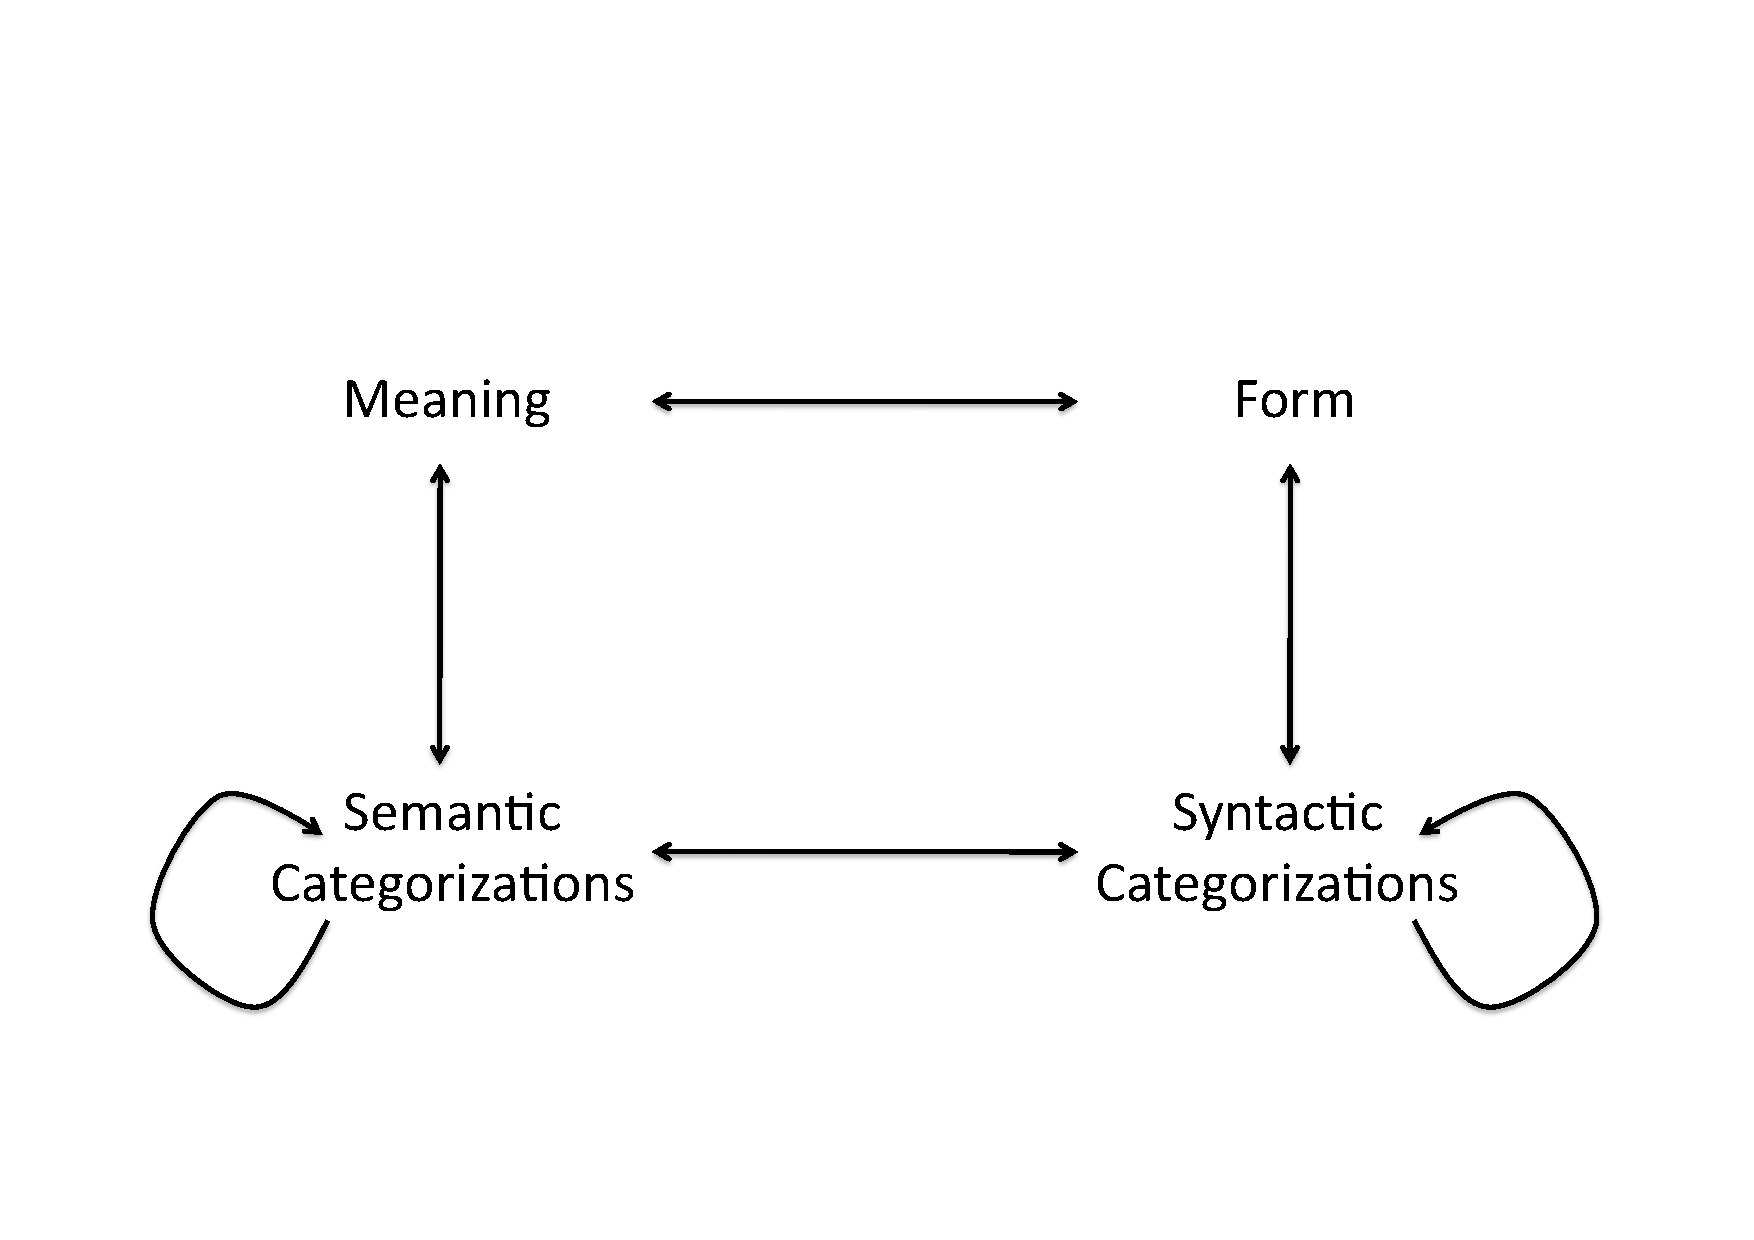
\includegraphics[width=0.7\columnwidth]{figs/grammar-square}
\end{center}
\caption[Grammar square]{The grammar square (figure 
adapted from \citealp{steels2011design}\index{Steels, L.}). Lexical constructions directly link meaning
and form, but grammatical construction go through an additional layer of
semantic and syntactic categorization}
\label{f:grammar-square}
\end{figure}

A number of studies on grammatical development focus on another aspect
of grammar which was not discussed in this book -- syntactic and semantic categorization \citep{steels2011phrasal}\index{Steels, L.}.
One of the functions of grammatical constructions is to re-categorize meaning 
and syntactic form in different levels of abstraction and specificity. 
A well worked out example for such processes is argument structure 
\citep{steels2002case,steels2007multi-level,vantrijp2008phd}. 
An example of a German phrase conveying the argument structure of a ``give event"
is the following 
\begin{example}
\gll Er gibt ihr ein Buch.
He.NOM gives her.DAT a book.ACC
\glt `He gives a book to her'
\glend
\end{example}

The phrase encodes that \emph{he} is the one who gives a book, and \emph{she} is 
the one who receives the book and \emph{the book} is the item that is given. 
The participants of the event are semantically re-categorized into semantic roles 
such as agent or patient. Syntactically, categorizations such as case (e.g. 
nominative, dative and accusative) or gender (e.g. female, masculine, neuter)
can be applied. The main purpose of semantic and syntactic re-categorization 
is to capture abstract semantic and grammatical mappings observed in 
natural language. The corresponding hypothesized constructions 
are consequently more abstract \citep{steels2011phrasal}\index{Steels, L.}. For instance,
an argument-linking construction does not depend on particular event participants
such as giver and givee, but rather relies on abstract semantic roles such
as agent and recipient.

In terms of evolution semantic and syntactic categorization are often connected. 
For instance, we know that case marking systems develop out of 
semantic roles \citep{blake1994case}\index{Blake, B.J.}. A fact that has been traced using computational
models of the evolutionary processes involved \citep{vantrijp2008phd}\index{van Trijp, R.}.
The line of research on case marking and semantic roles 
\citep{steels2002case,vantrijp2008phd}\index{Steels, L.}\index{van Trijp, R.} stresses an important
aspect of grammar that we can also see at work in German locative phrases.
Syntactic and semantic categorizations were used throughout the 
German locative grammar in the form of semantic and syntactic functions
and classes. These categorizations are important for organizing the grammar,
since abstract constructions build on top of them. An example of such a construction
in German is the postmodifier construction 
{\footnotesize\tt referring-expression--adverbial} which handles different kinds postmodifiers 
such as adverbs and prepositional phrases (see Section \ref{s:german-locative-phrases-syntax}). 

In the experiments in this book, semantic categorization is either given by the 
experimenter or directly derived from the type system used in semantic processing 
of IRL. Semantic categorization was designed by the experimenter for the 
German locative grammar. Great care was taken to ensure that semantic classes, 
functions and types are given so that the grammar can function properly. For grammar 
evolution, semantic categorization immediately follows from the type system 
used to represent categories, spatial relations and object classes.

An interesting direction for future work would certainly be to study the evolution of
syntactic and semantic categorization in spatial language. Semantic categories 
could start based on the type system implemented for spatial relations and
could gradually become more abstract -- the idea being that agents autonomously 
develop abstract constructions such as modeled for German locative phrases.

%\bibliographystyle{diss}
%\bibliography{papers,space}
%\end{document}

%
